\section{Primeiras gerações de redes móveis}

Devido à complexidade das redes móveis modernas, conhecer a evolução dessas redes se torna necessário para facilitar o seu entendimento. Originalmente, as redes móveis tinham o foco em comunicações de voz analógica, sendo uma extensão da rede de telefonia pública \textit{(Public Switched Telephone Network - PSTN)}, que operava com rede de roteamento de circuitos \cite{Cardoso2020}.
Entretanto, essas redes móveis foram adaptadas para transporte de dados com taxas de transmissão muito baixas, atingindo velocidades de até 2.4 kbps. Essas redes ficaram conhecidas como rede móvel de primeira geração (1G) \cite{vora2015evolution}.

Com a necessidade de evoluir as redes 1G, surge a segunda geração (2G), que provia um sinal com melhor qualidade, maiores taxas de transferência de dados e maior aproveitamento do espectro das ondas de rádio.
Todavia, essa tecnologia ainda mantinha seu foco em roteamento de circuitos.
Nessa geração, também surge o serviço de troca de mensagens curtas, conhecido como \textit{Short Message Service} (SMS).
Foi no 2G que a tecnologia de transporte de dados \textit{Global System for Mobile Communications} (GSM) foi inserida \cite{bhalla2010generations}.

Em 1998, inicia-se a parceria entre diversas organizações responsáveis pela criação dos padrões de telecomunicação denominada 3GPP\footnote{\url{https://www.3gpp.org/about-3gpp}}, que publica a \textit{Release 1999} no início do ano 2000.
Em redes móveis, \textit{releases} são conjuntos de recursos e especificações disponibilizadas a cada período, definindo os padrões a serem seguidos para a implementação dessas redes.
A \textit{Release 1999} descreve uma nova tecnologia de redes móveis, com foco em roteamento de pacotes.
Porém, essa tecnologia mantinha a compatibilidade com as tecnologias antigas, sendo denominada redes móveis de terceira geração (3G) \cite{3gpp.01.01}.

Inicialmente, o padrão definido para as redes 3G foi o \textit{Wide-Band Code-Divison Multiple Access} (WCDMA).
Entretanto, em 2002, o início do desenvolvimento do padrão \textit{High-Speed Downlink Packet Access} (HSDPA) é anunciado, suportando velocidades de transmissão teóricas de até 14 Mbps. Isso permitiria navegação na internet mais rápida, acesso a conteúdos de televisão diretamente no aparelho celular e chamadas de vídeo. O padrão HSDPA foi chamado de 3.5G e teve a sua especificação finalizada em 2004 \cite{Lamba2012}.

No final de 2008, a \textit{Release 8} é publicada pela 3GPP, especificando os requisitos para a tecnologia \textit{Long Term Evolution} (LTE), que viria para substituir a terceira geração de redes móveis.
Entretanto, essa especificação não preenchia os requisitos mínimos para ser considerada uma quarta geração de redes móveis, sendo assim conhecida como 3.9G \cite{delperal2018}.
Dentre as mudanças provindas desta nova tecnologia, é importante mencionar a remoção do suporte à roteamento de circuitos, fazendo com que essa geração usasse apenas roteamento de pacotes sobre IP para todo o tráfego de informações na rede.

Toda a informação de áudio de ligações telefônicas era trafegada sobre a rede de roteamento de circuitos nas gerações anteriores ao LTE.
Com a remoção dessa tecnologia no LTE, foi necessário desenvolver um novo protocolo, surgindo assim o \textit{Voice over LTE} (VoLTE).
O VoLTE, assim como a tecnologia \textit{Voice over IP} (VoIP), trafega os dados de voz de ligações telefônicas sobre a rede de roteamento de pacotes, permitindo que as operadoras de redes móveis pudessem continuar oferecendo o serviço de ligações telefônicas para seus clientes. Nesta época, esse serviço era o mais rentável para as operadoras \cite{Yi2012}. 

Visando preencher os requisitos mínimos para a criação da quarta geração de redes móveis (4G), no início de 2011 é publicada a \textit{Release 10} pela 3GPP, criando assim a tecnologia \textit{LTE-Advanced} (LTE-A) \cite{3gpp.21.201}.
O 4G prometia velocidades de \textit{download} de pico de até 1Gbps e velocidades de \textit{upload} de pico de até 100Mbps.
Atingir tais velocidades só era possível graças à remoção do suporte ao roteamento de circuitos que ocorreu no 3.9G.

Antes do surgimento do LTE, existiam apenas 3 componentes na rede. Um era o equipamento de usuário, denominado \textit{User Equipment} (UE), sendo esse o dispositivo móvel. Outro componente era a rede de acesso via rádio, ou \textit{Radio Access Network} (RAN), denominada na tecnologia 3G de \textit{Universal Mobile Telecommunications System (UMTS) Terrestial Radio Network} (UTRAN), que englobava a estação de rádio base, chamada de \textit{Node B} (NB). Por fim, o terceiro componente era o núcleo da rede, ou \textit{Core Network} (CN), que no 3G era denominado \textit{UMTS Core Network} \cite{Miah2002}.
No entanto, a especificação da rede LTE trouxe uma melhor separação dos seus componentes do núcleo da rede, denominado \textit{Evolved Packet Core} (EPC) nessa geração, além de renomear a RAN para \textit{Evolved UTRAN} (E-UTRAN), chamando a estação base de \textit{Evolved Node B} (eNodeB).
O EPC foi separado em 4 elementos, sendo eles o \textit{Serving Gateway (Serving GW)}, o \textit{Packet Data Network Gateway (PDN GW)}, o \textit{Mobility Management Entity} (MME) e o \textit{Home Subscriber Server} (HSS) \cite{3gpp.23.214}.

\section{Redes 5G}

Em 2017, a 3GPP publica a versão inicial da \textit{Release 15}, com as definições da quinta geração de redes móveis, o 5G \cite{3gpp.21.205}.
Assim como nas gerações anteriores, o 5G visava introduzir melhorias na capacidade de transmissão de dados da RAN e redução da latência de comunicação entre o UE e a RAN.
Entretanto, essa geração teve como objetivo criar uma rede mais dinâmica e com maior flexibilidade em relação ao LTE.
Nessa geração também houve a integração com tecnologias de comunicação sem fios não-3GPP, que enquadram dispositivos denominados de \textit{Internet of Things} (IoT).

A \textit{Release 15} também introduziu as arquiteturas de rede 5G \textit{Non-Stand Alone} (NSA) e 5G \textit{Stand Alone} (SA).
Na arquitetura NSA, o núcleo da rede 4G é utilizado para a autenticação e comunicação dos dispositivos 5G, substituindo-se a E-UTRAN pela \textit{5G New Radio} (5GNR) e, consequentemente, a eNodeB pela gNodeB.
A rede NSA é considerada uma rede de transição entre o 4G e o 5G, pois o custo de implementação é baixo em ambientes onde já existe cobertura 4G das operadoras.

Por outro lado, a arquitetura SA introduziu um novo núcleo da rede, denominado de \textit{5G Core} (5GC).
De acordo com a especificação da 3GPP, o 5GC é um conjunto de componentes interconectados através de uma camada de serviços. Cada componente tem seu grupo específico de responsabilidades por consumir e prover serviços de e para outros elementos do sistema 5G, através de uma \textit{Application Programming Interface} (API).

A quinta geração de redes móveis também trouxe uma nova arquitetura do núcleo da rede, ilustrada em alto nível na Figura \ref{fig:5Gcore}. Os principais componentes dessa rede são o \textit{Access and Mobility Management Function} (AMF), o \textit{Session Management Function} (SMF) e o \textit{User Plane Function} (UPF).
O AMF é responsável por garantir que o processo de comunicação ocorra de maneira coesa e transparente, considerando a mobilidade do usuário como principal fator.
O SMF é responsável por estabelecer, modificar e liberar as sessões de cada equipamento de usuário, além de requisitar a alocação de um endereço de IP para esses UEs.
O UPF é o responsável pelo processamento e encaminhamento dos dados provindos dos UEs. Esses componentes serão discutidos com maior profundidade na subseção \ref{sub:components}.

\begin{figure}[!ht]
    \centering
    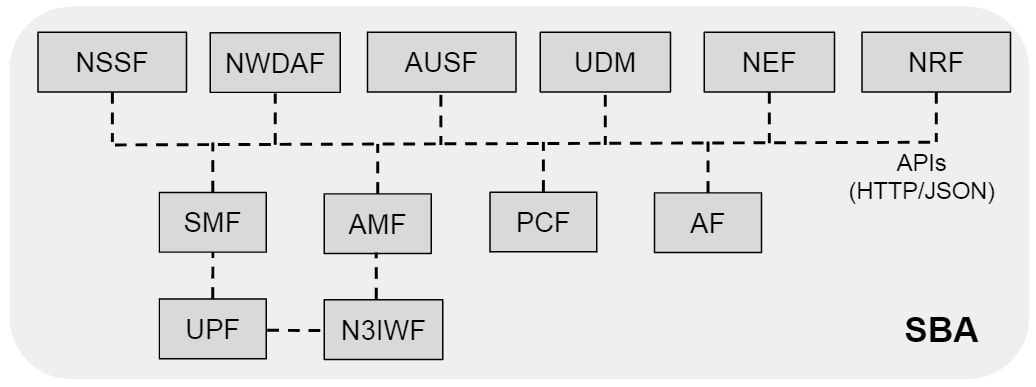
\includegraphics[width=1\textwidth]{TG2/Chapters/Background/Figures/Background-Core5G.png}
    \captionsource{Core 5G software components.}{\cite[p.~15]{Cardoso2020}}
    \label{fig:5Gcore}
\end{figure}

Os demais nove componentes do núcleo do 5G realizam uma variedade de funções.
O \textit{Authentication Server Function} (AUSF) é a função responsável por prover os serviços de autenticação dos UEs.
O \textit{Unified Data Management} (UDM) gerencia as informações dos usuários conectados na rede.
O \textit{Network Repository Function} (NRF) é um repositório que lista todas as funções de rede disponíveis em sua instância do núcleo do 5G.
O \textit{Policy Control Function} (PCF) é o responsável por controlar o comportamento da rede, aplicando políticas de segurança e controle.
O \textit{Network Slice Selection Function} (NSSF) é o componente responsável por controlar os \textit{slices} da rede para cada UE.
O \textit{Network Exposure Function} (NEF) é responsável por expor eventos internos relacionados aos UEs.
O \textit{Network Data Analytics Function} (NWDAF) é a função responsável por coletar e analisar dados provindos dos outros componentes da rede, incluindo informações dos usuários.
O \textit{Application Function} (AF) é um componente genérico que interage com os outros componentes no intuito de melhorar a qualidade do serviço para o usuário.
O \textit{Non-3GPP InterWorking Function} (N3IWF) é o responsável por integrar dispositivos não-3GPP com a rede 5G.

\subsection{Protocolos NAS e NGAP e Sessões de PDU}

Os protocolos \textit{Non-Access Stratum} (NAS) e \textit{NG Application Protocol} (NGAP) são essenciais para a comunicação entre o núcleo da rede, a RAN e o UE através do plano de controle.
As sessões de \textit{Packet Data Unit} (PDU) são importantes para garantir o funcionamento do plano de usuário da rede 5G.
A Figura \ref{fig:5Gprotocols} representa a arquitetura de uma rede 5G, exibindo os protocolos NAS e NGAP e as sessões de PDU entre o equipamento de usuário, a gNodeB e o núcleo da rede.

\begin{figure}[!ht]
    \centering
    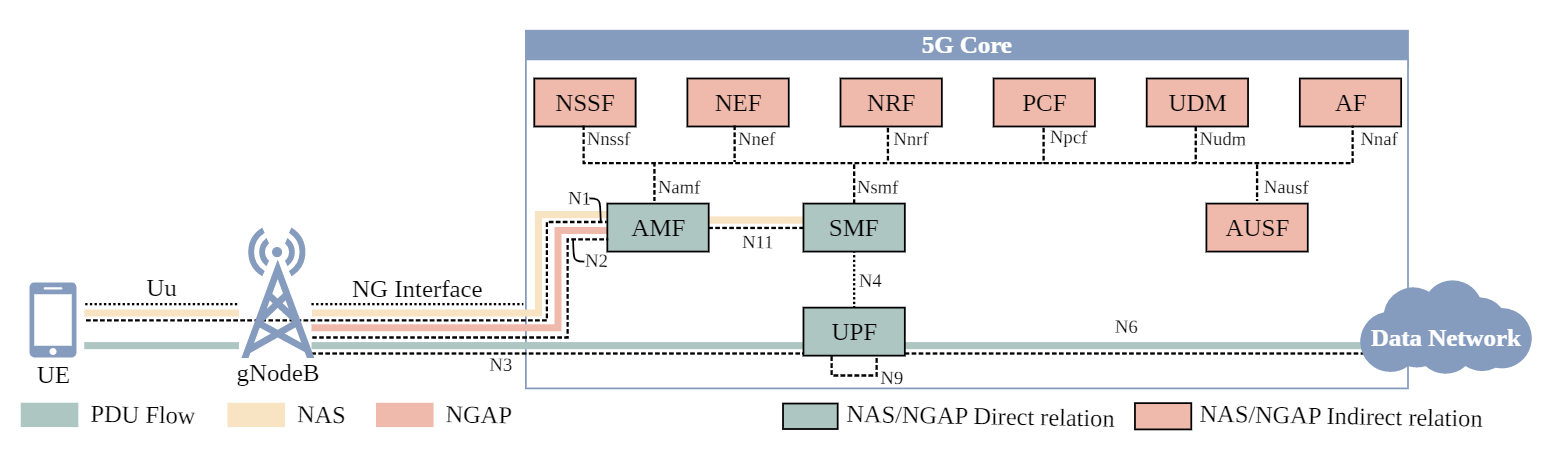
\includegraphics[width=1\textwidth]{TG2/Chapters/Background/Figures/Background-5GSystemProtocols.png}
    \captionsource{5G Core (5GC) Service-based Architecture (SBA).}{\cite[p.~3]{Dominato2021}}
    \label{fig:5Gprotocols}
\end{figure}

O protocolo NAS é usado para fazer a comunicação entre o UE e a função do núcleo AMF, tanto para dispositivos 3GPP quanto não-3GPP. A principal função do protocolo NAS é dar suporte à mobilidade do equipamento de usuário, incluindo procedimentos como autenticação, identificação e atualização das configurações genéricas do UE. O NAS também é responsável por suportar os procedimentos de gerenciamento de sessões, para estabelecer e manter a conexão de dados entre o UE e a rede de dados \cite{3gpp.24.501}. Esse protocolo também é o responsável por fazer a autenticação e gerenciar a conexão da gNodeB com o núcleo da rede.

O protocolo NGAP é o protocolo padrão para a comunicação do plano de controle entre a RAN e o núcleo da rede. O NGAP suporta os procedimentos de gerenciamento de interfaces, transporte das mensagens do protocolo NAS, gerenciamento de contexto do UE e das sessões de PDU. O gerenciamento de interfaces é o responsável por estabelecer e manter a conexão entre os componentes do núcleo da rede, onde as mensagens dos protocolos NAS e NGAP são transportados. O Protocolo NGAP é responsável por encapsular e transportar as mensagens NAS, provindas do UE, entre a RAN e o AMF. O gerenciamento de contexto do UE provê informações dos UEs para a RAN, como informações de segurança, lista de restrições de mobilidade e capacidade do rádio do UE. O gerenciamento das sessões de PDU é responsável por gerenciar os fluxos das unidades de pacotes de dados entre o núcleo da rede e a RAN, estabelecendo a interface de rádio utilizada para tráfego de controle e dados dos UEs \cite{3gpp.38.413}.

As sessões de PDU são responsáveis por prover a conexão fim-a-fim para o plano de usuário entre o UE e a rede de dados externa, através da função de rede UPF.
O fluxo de dados trafegado através das sessões de PDU é chamado de fluxo PDU e seus pacotes de dados são encapsulando sobre o protocolo de rede \textit{User Datagram Protocol} (UDP) \cite{3gpp.38.415}.

\subsection{Principais componentes da Rede 5G}
\label{sub:components}

Dentro do núcleo da rede, os componentes AMF, SMF e UPF são os responsáveis por gerenciar todo o tráfego de informações provindos da RAN.
O AMF é a porta de entrada do núcleo da rede em relação ao plano de controle.
Sendo assim, todo o tráfego dos protocolos NAS e NGAP provindos da RAN é direcionado para essa função do núcleo da rede.
Quando uma nova gNodeB inicia o processo de conexão com um núcleo existente, a autenticação e o estabelecimento da conexão é feito através de mensagens trocadas que utilizam o protocolo NAS entre a RAN e o AMF.
Após estabelecida a conexão, uma mensagem é enviada da RAN para o SMF, indiretamente através do AMF, utilizando o protocolo NAS, para que o SMF tenha conhecimento da gNodeB e possa gerenciar sua sessão.

Estando a RAN operacional, dispositivos 3GPP e não-3GPP dentro da área de cobertura da antena poderão iniciar sua conexão com essa rede 5G. Um dispositivo 3GPP, ao iniciar a conexão com essa rede 5G, troca mensagens com a RAN através do protocolo NAS. A RAN encapsula essas mensagens para o protocolo NGAP e encaminha para o núcleo da rede. O AMF, comunicando-se com os demais componentes da rede, autentica o UE através de um fluxo de informações definido na \textit{Release 15} do 3GPP \cite{3gpp.29.509}. Após concluir a autenticação do UE, o SMF se torna o responsável por gerenciar a sessão do equipamento de usuário. Um fluxo de dados PDU é estabelecido entre o UE e a função do núcleo UPF, que é responsável por gerenciar e encaminhar os pacotes de dados provindos dos UEs.

O UPF é a função do núcleo da rede 5G responsável por ser o ponto de conexão do núcleo da rede com qualquer rede externa.
É o UPF que encaminha os pacotes de dados provindos do UE através das sessões de PDU para a rede externa, sendo o responsável pelo roteamento de pacotes entre a rede externa e os diversos UEs conectados nessa rede 5G.
Essa função do núcleo da rede 5G aloca os endereços de IP para os UEs quando requisitado pelo SMF \cite{3gpp.23.501}.
O UPF também é responsável por coletar métricas de qualidade de serviço (QoS) do plano de usuário que serão usadas na função NWDAF \cite{3gpp.23.548}.

\section{Testes em rede móveis definidas por software}

Segundo \cite[p.~2, tradução nossa]{Bertolino2003}, ``teste de software consiste na verificação dinâmica do comportamento de um programa em um conjunto finito de casos de teste, adequadamente selecionados do domínio de execuções geralmente infinitas, em relação ao comportamento esperado especificado".
Com relação ao comportamento das redes sem fios implementadas em software, é importante executar testes para garantir que o funcionamento da rede esteja dentro do esperado.
Dentre os tipos de testes que podem ser executados em cima de implementações de redes 5G \textit{open source}, os que se destacam são os testes de conformidade, robustez e desempenho, como descrito em \cite{Dominato2021} e \cite{Zhang2019ASO}.

\subsection{Testes de Conformidade}

De acordo com \cite{Sarikaya1989}, teste de conformidade é definido como a atividade de teste realizada com o objetivo de verificar as capacidades e o comportamento de uma implementação em teste em relação aos requisitos de conformidade fornecidos no padrão de protocolo.
Os resultados dos testes de conformidade são do tipo lógico, sendo verdadeiro no caso onde a implementação em teste seja aprovada e falso no caso contrário.
Dessa forma, o uso de testes de conformidade em redes 5G é importante para verificar se a implementação da rede móvel se comporta de acordo com a especificação da 3GPP em casos onde o equipamento de usuário execute corretamente as operações descritas.

\cite{Rayner1987} divide o grupo de testes de conformidade em quatro categorias: testes básicos de interconexão, testes de capacidade, testes de comportamento e testes de resolução de conformidade.
Os testes básicos de interconexão são feitos para detectar quaisquer casos graves de não conformidade com a especificação do sistema.
Os testes de capacidade verificam se as capacidades observáveis da implementação em teste estão de acordo com os requisitos de conformidade estática da especificação. Os testes de conformidade estática são executados sobre o código fonte da aplicação.
Os testes de comportamento verificam a implementação da forma mais abrangente possível para ver se a implementação está de acordo com os requisitos de conformidade dinâmica da especificação. Os testes de conformidade dinâmica são realizados durante ou após a execução da implementação.
Os testes de resolução de conformidade examinam em profundidade requisitos específicos na implementação, verificando se a implementação se comporta exatamente como a especificação destes requisitos.

\subsection{Testes de Robustez}

Segundo \cite[p.~64, tradução nossa]{IEEE.Standard.Glossary}, robustez é definida como ``o grau em que um sistema ou componente pode funcionar corretamente na presença de entradas inválidas ou condições ambientais estressantes".
Os resultados dos testes de robustez também são do tipo lógico, sendo verdadeiro no caso onde a implementação em teste seja aprovada e falso no caso contrário.
Sendo assim, o teste de robustez no núcleo de redes móveis verifica o comportamento da rede em situações atípicas. \cite{Dominato2021} dividem o grupo de testes de robustez em um subgrupo de testes, que envolve testes de registro, de autenticação e de segurança, além de testes específicos para cada protocolo e função de rede do núcleo que serão detalhados na Subseção \ref{subsec:Dominato}.

\subsection{Testes de Desempenho}

Os testes de desempenho são importantes para validar o funcionamento da rede em uma carga alta de trabalho, o que representa uma situação de sobrecarga de uso da rede, o que pode causar mal funcionamento da rede e, em situações mais críticas, uma interrupção total do serviço.
Para a execução de testes de desempenho, costuma-se usar aplicações de referência, chamados de \textit{benchmarks}.
Os \textit{softwares} de \textit{benchmark} são aqueles que utilizam os mesmos parâmetros de entrada para avaliar o desempenho de diferentes sistemas ou serviços \cite{Boano2018}.
Sendo assim, o usuário pode comparar as métricas obtidas na execução com métricas coletadas de outras execuções em diferentes sistemas ou serviços e avaliar o desempenho do teste.

Para a avaliação dos testes de desempenho em redes móveis em software, \cite{Lee2021} utilizam dois grupos de métricas.
O primeiro grupo engloba métricas de desempenho de rede: taxa de transferência de dados, latência e perda de pacotes.
O segundo grupo é composto por métricas de desempenho de \textit{hardware}: carga do processador, tempo de execução e tempo de processador.

Em relação as métricas de desempenho de rede, a taxa de transferência é definida por \cite[p.~77, tradução nossa]{IEEE.Standard.Glossary} como ``a quantidade de trabalho que pode ser realizada por um sistema ou componente de computador em um determinado período de tempo''. Sendo assim, a taxa de transferência de dados em uma rede pode ser caracterizada como a quantidade de dados movida com sucesso de um lugar para outro em um determinado período de tempo.
\cite[p.~43, tradução nossa]{IEEE.Standard.Glossary} definem latência como ``o intervalo de tempo entre o instante em que uma unidade de controle de instrução emite uma chamada de dados e o instante em que a transferência de dados é iniciada.'' Se tratando de redes de computadores, latência se refere ao tempo que um pacote de dados leva para ser gerado no emissor, transmitido pela rede, e recebido e decodificado no receptor.
\cite{Bhadra2015} definem perda de pacotes como a falha de pacotes de dados ao chegar a um destino específico. Esse tipo de falha tende a afetar os mais diversos tipos de comunicação e podem produzir dados incorretos no destinatário.

Quanto a métricas de desempenho do \textit{hardware}, a carga do processador, também conhecido como \textit{Central Processing Unit} (CPU), é definida como o número de processos que estão sendo executados por uma CPU ou estão aguardando para serem executados \cite{Sebastian2014}.
\cite[p.~242, tradução nossa]{Patterson2014-qv} definem tempo de execução como ``o tempo total necessário para o computador concluir uma tarefa, incluindo acessos ao disco, acessos à memória, atividades de entrada e saída de dados, sobrecarga do sistema operacional, tempo de execução da CPU e assim por diante''. Já o tempo de processador é definido como somente o tempo que a CPU gasta computando uma tarefa específica \cite{Patterson2014-qv}.
